% Created 2022-04-02 Sat 18:41
% Intended LaTeX compiler: pdflatex
\documentclass[a4paper, 11pt]{article}
\usepackage[utf8]{inputenc}
\usepackage[T1]{fontenc}
\usepackage{graphicx}
\usepackage{longtable}
\usepackage{wrapfig}
\usepackage{rotating}
\usepackage[normalem]{ulem}
\usepackage{amsmath}
\usepackage{amssymb}
\usepackage{capt-of}
\usepackage{hyperref}
\usepackage[margin=.75in]{geometry}
\usepackage{amsmath}
\usepackage{subfig}
\usepackage[demo]{graphicx}
\usepackage[nodisplayskipstretch]{setspace}
\author{Mick Harrigan}
\date{04/02/2022}
\title{\textbf{CMPE320 Project 3}\\\medskip
\large \textbf{The Central Limit Theorem: The Magic of Large Numbers}}
\hypersetup{
 pdfauthor={Mick Harrigan},
 pdftitle={\textbf{CMPE320 Project 3}},
 pdfkeywords={},
 pdfsubject={},
 pdfcreator={Emacs 27.2 (Org mode 9.6)}, 
 pdflang={English}}
\begin{document}

\maketitle
\setstretch{1.5}
\section{Introduction}
\label{sec:org058ef41}
This project uses different types of random variables to show the effects of the CLT on real datasets.
The effects of this theorem are simply stated that the sum of many different random variables tends towards a gaussian distribution with a mean equivalent to the sum of the means, and variance equivalent to the sum of the variances. The findings below agree with this notion and are shown as such.
\section{Simulation and Discussion}
\label{sec:org3d0db69}
\subsection{Sum of Independent, Identically Distributed Random Variables from \(U(0,1)\)}
\label{sec:org0023b57}
For the sum of the iid variables in this sample the generalized shape is going to be based on the generation of \(100,000\) random numbers between \(0\) and \(1\). Because of this being a uniform distribution, the analytical mean is found to be \(0.5\).
The variance of the same set of data is found to be \(0.833\). With these pieces of information the CLT can be upheld by summing each of the means and variances for each trial of different \(N\) values. These are illustrated below in Figure \ref{fig:UniformSubFig}.

\pagebreak

\begin{figure}
    \centering
    \subfloat[Sum of 2 Uniform Distributions]{{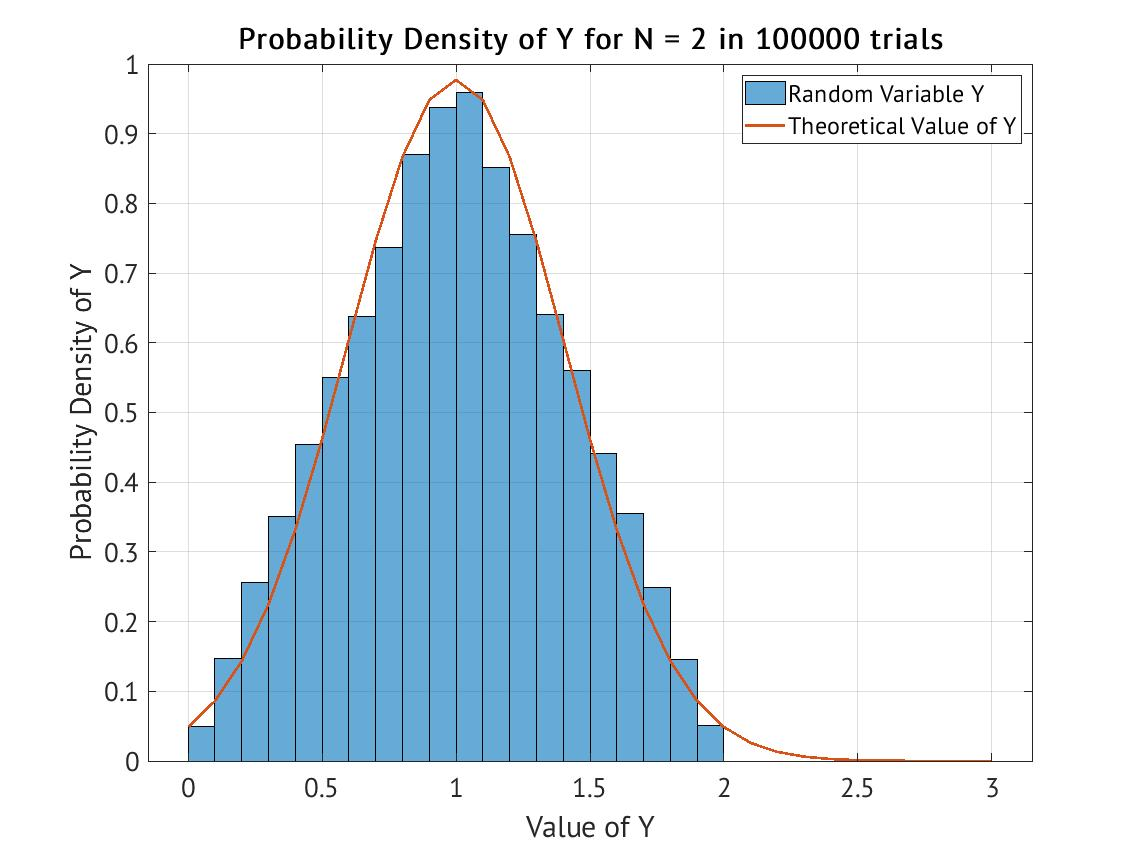
\includegraphics[width=0.5\textwidth]{./Images/UniformFig1.jpg} }}
    \subfloat[Sum of 6 Uniform Distributions]{{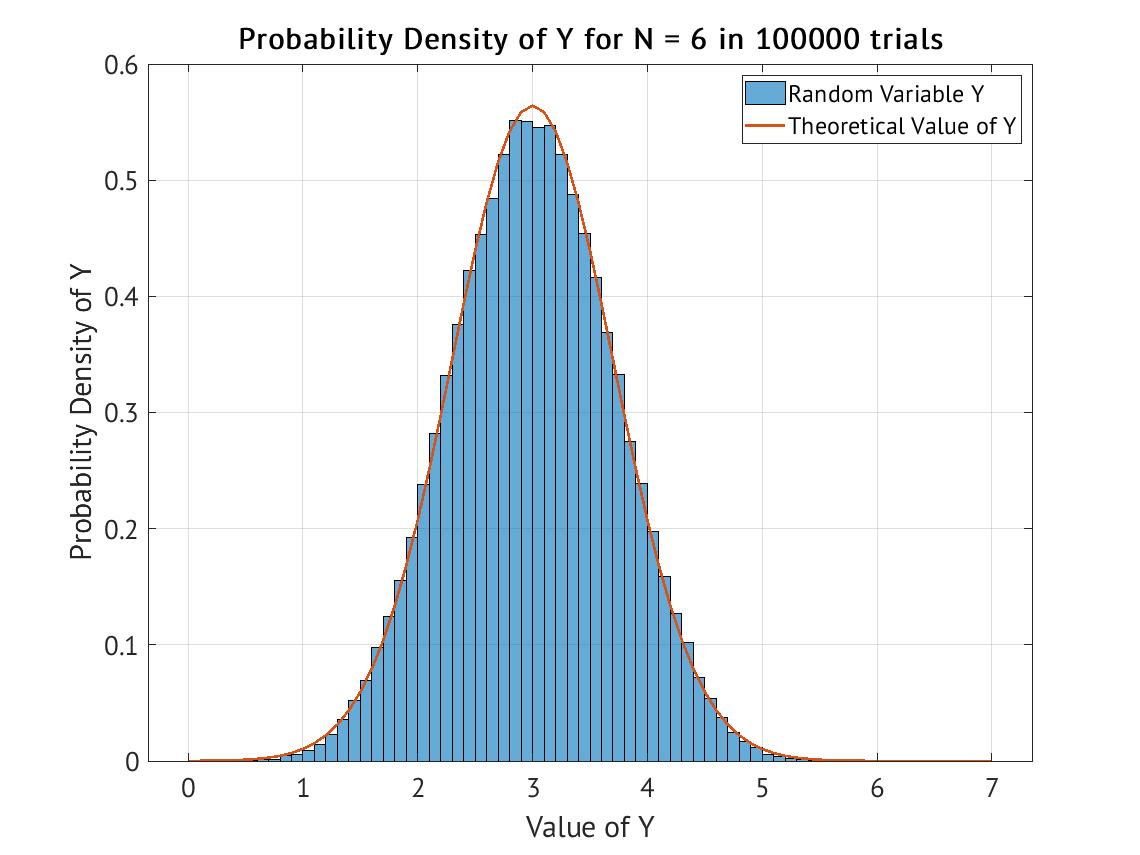
\includegraphics[width=0.5\textwidth]{./Images/UniformFig2.jpg} }} \\
    \subfloat[Sum of 12 Uniform Distributions]{{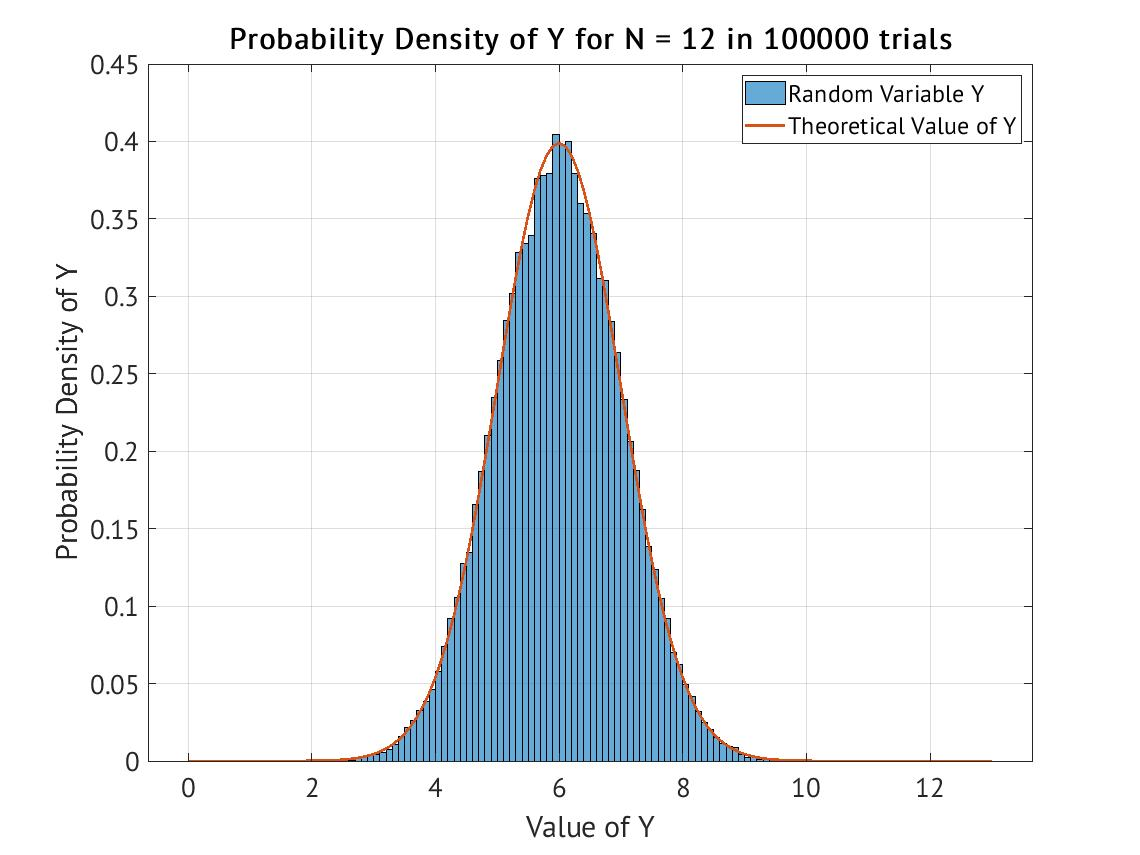
\includegraphics[width=0.5\textwidth]{./Images/UniformFig3.jpg} }}
\caption{\label{fig:UniformSubFig}Sum of iid Uniform Random Variables for N = 2,6,12}
\end{figure}

\noindent
Given the formerly calulated values of \(\mu = 0.5\) and \(\sigma^2 = 0.833\), the reflected outputs for different amounts of summed random variables follows suit with the output means and variances being \(N\) times \(\mu\) and \(\sigma^2\) respectively.
The graphs show this with obvious means of \(N\) divided by \(2\), and greater variance from the mean as \(N\) increases, equivalent to \(N\) divided by \(12\).

\medskip
\noindent
In each graph there is an appropriate Gaussian curve plotted above the histograms. These use the analytical values calulated for the mean and variance to show what the expected output of this function is to be, given that the CLT is true.

\medskip
\noindent
The comparison between analytical and measured mean and variance for each of the trials can be summarized below in Table \ref{tab:UniformTable}.

\begin{table}[htbp]
\caption{\label{tab:UniformTable}Simulated and Analytical Mean and Variance for each trial of N}
\centering
\begin{tabular}{|c|c|c|c|c|}
\hline
N & Analytical Mean & Simulated Mean & Analytical Variance & Simulated Variance\\
\hline
2 & 1 & 1 & 1.6667 & 0.16649\\
6 & 3 & 3.003 & 0.5 & 0.49669\\
12 & 6 & 6.0008 & 1 & 1.0008\\
\hline
\end{tabular}
\end{table}

\noindent
This shows that even given a very small amount of trials the accuracy of the approach to Gaussian is very high. Then, in this case at least, the CLT does hold up. With this distribution the CLT makes sense given that as \(N\) increases, thus would the mean, and as there are more values being used as each trial, the relative amount of differences within each point increases as well which leads to a greater variance as well.


\subsection{Sum of Independent, Identically Distributed Discrete Random Variables}
\label{sec:org23375f9}
The sum of \(N\) trials of rolling a fair 8 sided die is going to follow a similar output to that of Section \ref{sec:org0023b57}. This is because of the CLT once again and the subfigures of Figure \ref{fig:DiscreteSubfig} show this below.

\pagebreak
\begin{figure}
    \centering
    \subfloat[Sum of 2 Discrete Distributions]{{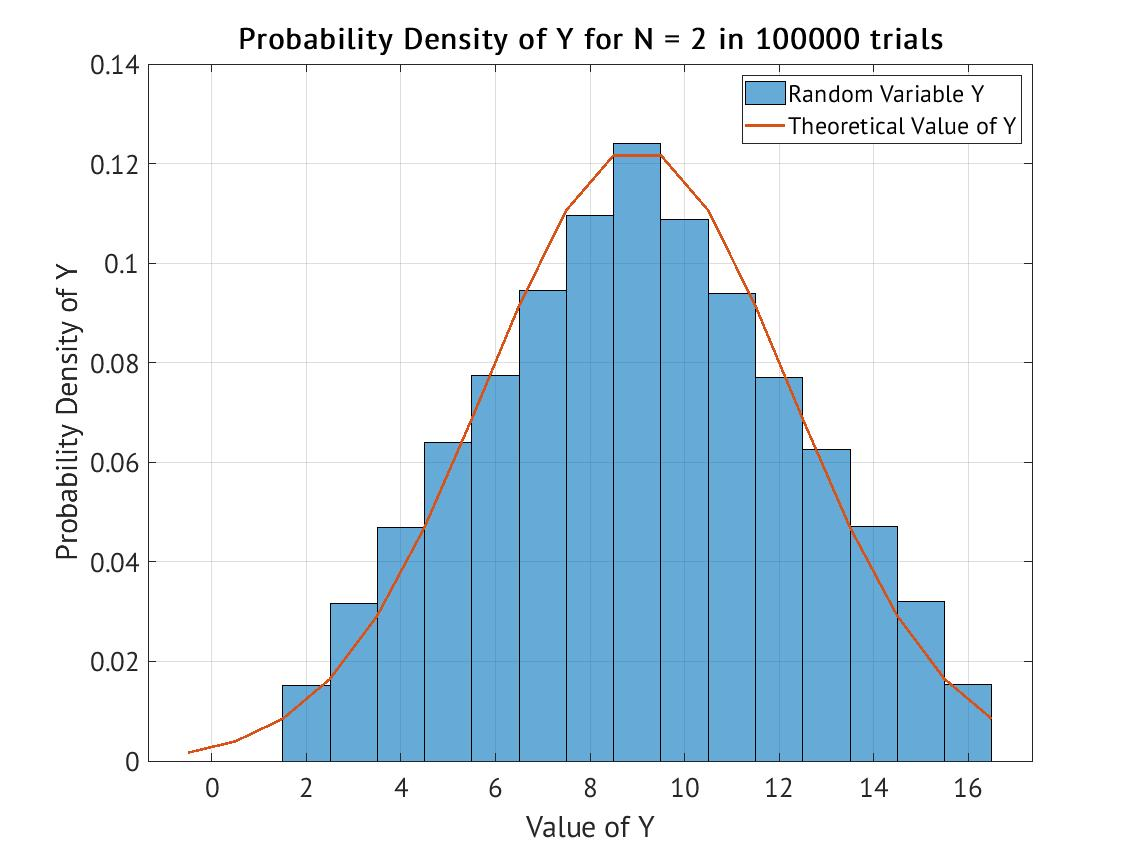
\includegraphics[width=0.5\textwidth]{./Images/DiscreteFig1.jpg} }}
    \subfloat[Sum of 20 Discrete Distributions]{{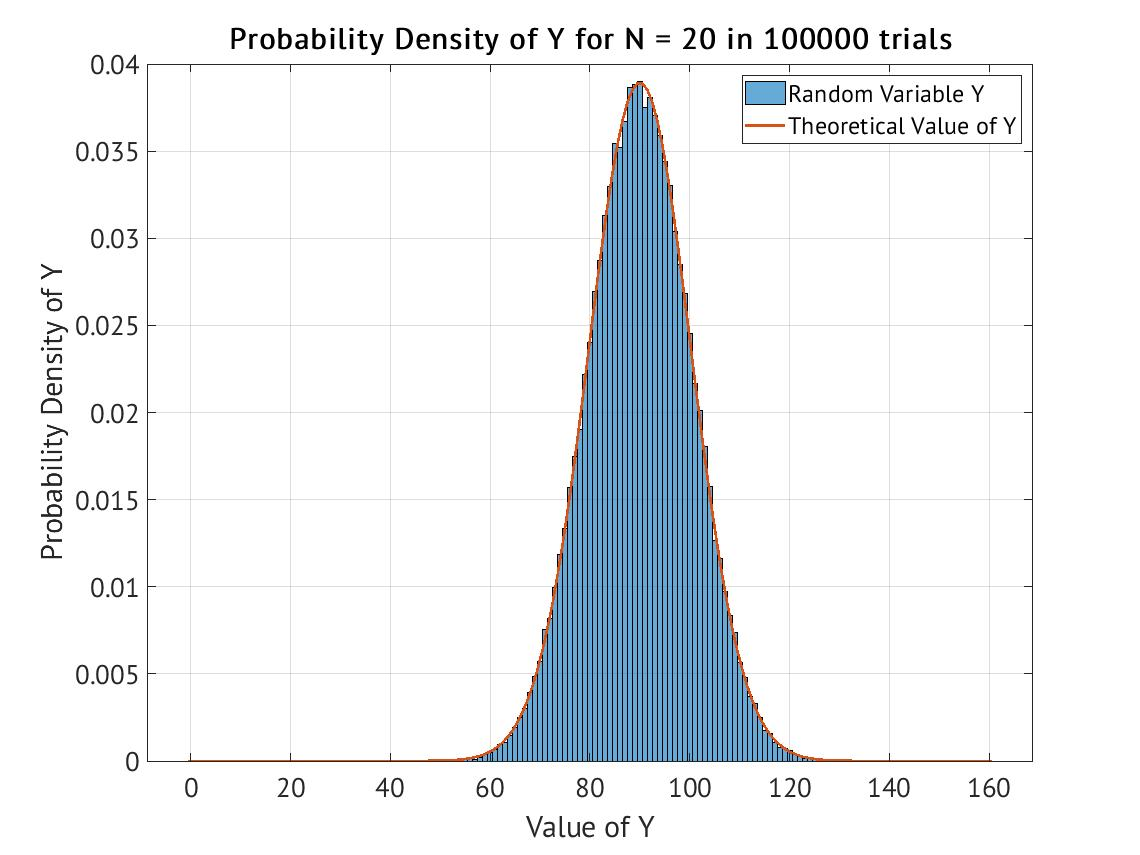
\includegraphics[width=0.5\textwidth]{./Images/DiscreteFig2.jpg} }} \\
    \subfloat[Sum of 40 Discrete Distributions]{{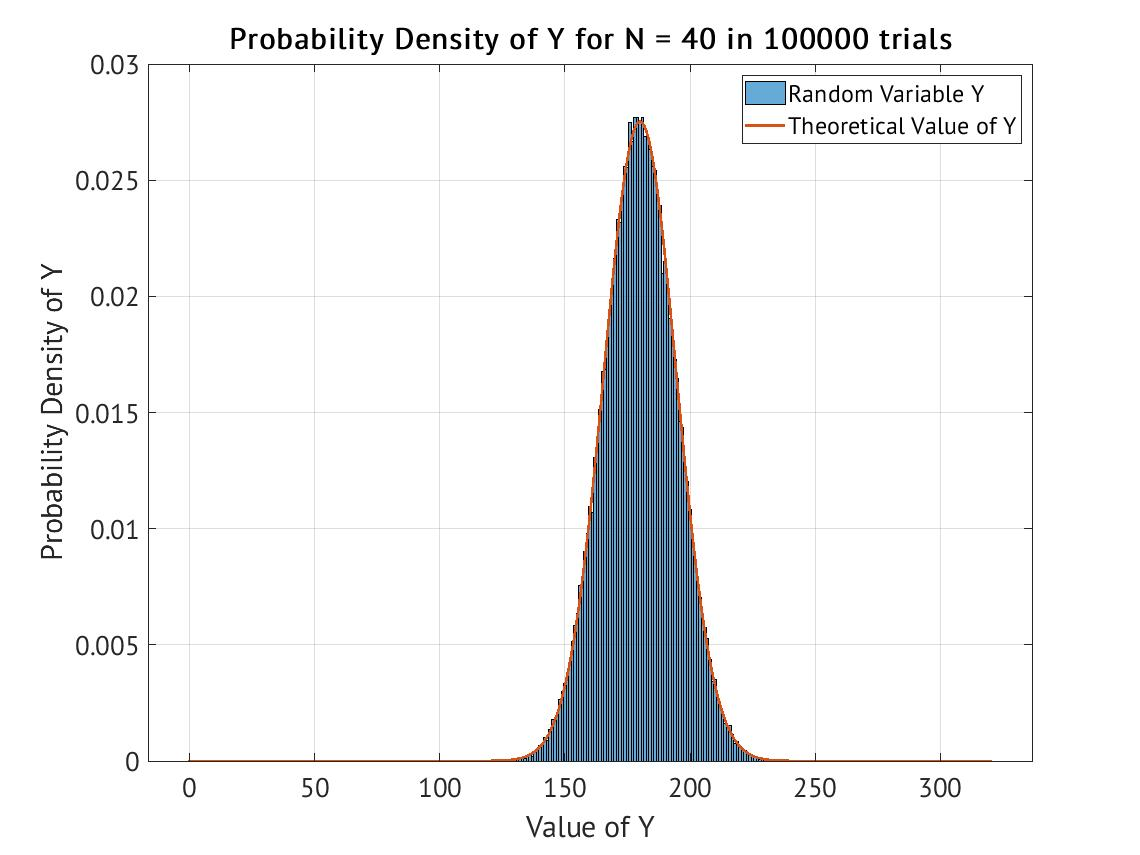
\includegraphics[width=0.5\textwidth]{./Images/DiscreteFig3.jpg} }}
\caption{\label{fig:DiscreteSubfig}Sum of iid Discrete Random Variables for N = 2,20,40}
\end{figure}

\noindent
In Figure \ref{fig:DiscreteSubfig} subfigure a, the bounds are most easily seen compared to the other 2 graphs. The low end of the histogram being \(2\), and the high end being \(16\). These values are important given that there is no way for the max (in the case of \(N = 2\)) value to be greater than \(2 \times 8\), as that is the max value of each die. The same applies to the low end of the histogram in that the minimum value is when each die is at it's minimum, \(2 \times 1\).

\pagebreak
\noindent
Given that the distribution of the random variables of \(X\) are discrete, the values are inherently between the values of \(1\) and \(8\). The mean of this variable is found as the probability of each possible outcome times the outcome itself.
Because this is a fair \(8\) sided die, the probability for each side is \(1/8\), and the values are the sum of each of the sides, \(1+...+8\).
Thus the following is the expected value of \(X\).

\begin{flalign}
\label{eqn:DiscreteMean}
    \mu &= \frac{1}{8} \sum_{k=1}^{8}{k} \\
        &= \frac{1 + 2 + 3 + 4 + 5 + 6 + 7 + 8}{8} \\
        &= \frac{36}{8} \rightarrow 4.5
\end{flalign}

\noindent
Finding the variance of the same random variable can be done through subtracting the square of the mean from the mean square.

\begin{equation}
    \sigma^2 = E[X^2] - (E[X]^2)
\end{equation}

\noindent
Calculating the mean square is similar to the process of the mean, shown in Equation \ref{eqn:DiscreteMean}. This calculation is shown below.

\begin{flalign}
\label{eqn:DiscreteMeanSquare}
    E[X^2]  &= \frac{1}{8} \sum_{k=1}^{8}{k^2} \\
            &= \frac{1^2 + 2^2 + 3^2 + 4^2 + 5^2 + 6^2 + 7^2 + 8^2}{8}  \\
            &= \frac{204}{8} \rightarrow 25.5
\end{flalign}


\noindent
With both the mean and the mean square, the variance is thus found as shown in Equation \ref{eqn:DiscreteVar}.

\begin{equation}
\label{eqn:DiscreteVar}
    \sigma^2    &= E[X^2] - (E[X]^2) \\
                &= 25.5 - (4.5)^2 \\
                &= 5.25
\end{equation}

\noindent
Using both the calculated mean and variance in Equations \ref{eqn:DiscreteMean} and \ref{eqn:DiscreteVar}, the analytical function for each value of \(N\) multiplies \(N\) by the mean and variance to find the applicable mean and variance, as stated by the CLT.
Once again, in each subfigure of Figure \ref{fig:DiscreteSubfig} this is seen as the mean for each is \(4.5\) times \(N\), and each having a greater and greater range of output values due to the increases in each mean and variance of the different \(N\) values.

\medskip
\noindent
With the data generated, comparing the calculated and analytical values leads to a similar conclusion to that from Section \ref{sec:org0023b57}, as seen below in Table \ref{tab:DiscreteTab}.

\begin{table}[htbp]
\caption{\label{tab:DiscreteTab}Simulated and Analytical Mean and Variance for each trial of N}
\centering
\begin{tabular}{|c|c|c|c|c|}
\hline
N & Analytical Mean & Simulated Mean & Analytical Variance & Simulated Variance\\
\hline
2 & 9 & 8.9955 & 10.5 & 10.5242\\
20 & 90 & 89.9882 & 105 & 104.471\\
40 & 180 & 179.9561 & 210 & 210.4184\\
\hline
\end{tabular}
\end{table}

\subsection{Sum of Independent, Identically Distributed Random Variables from \(p_X(x)=0.5e^{-0.5x}\)}
\label{sec:org69fa2f4}
This case uses a much more different function to show the breadth of the CLT's applications. The past 2 random variables have been generally simple and not following a real function, unlike the current case.
The function for this case is \(p_X(x)=0.5e^{-0.5x}\), and upon initial thought the past events might not seem as probable.
This worry is denied below in Figure \ref{fig:ExpSubFig}.

\pagebreak
\begin{figure}
    \centering
    \subfloat[Sum of 5 Exponential Distributions]{{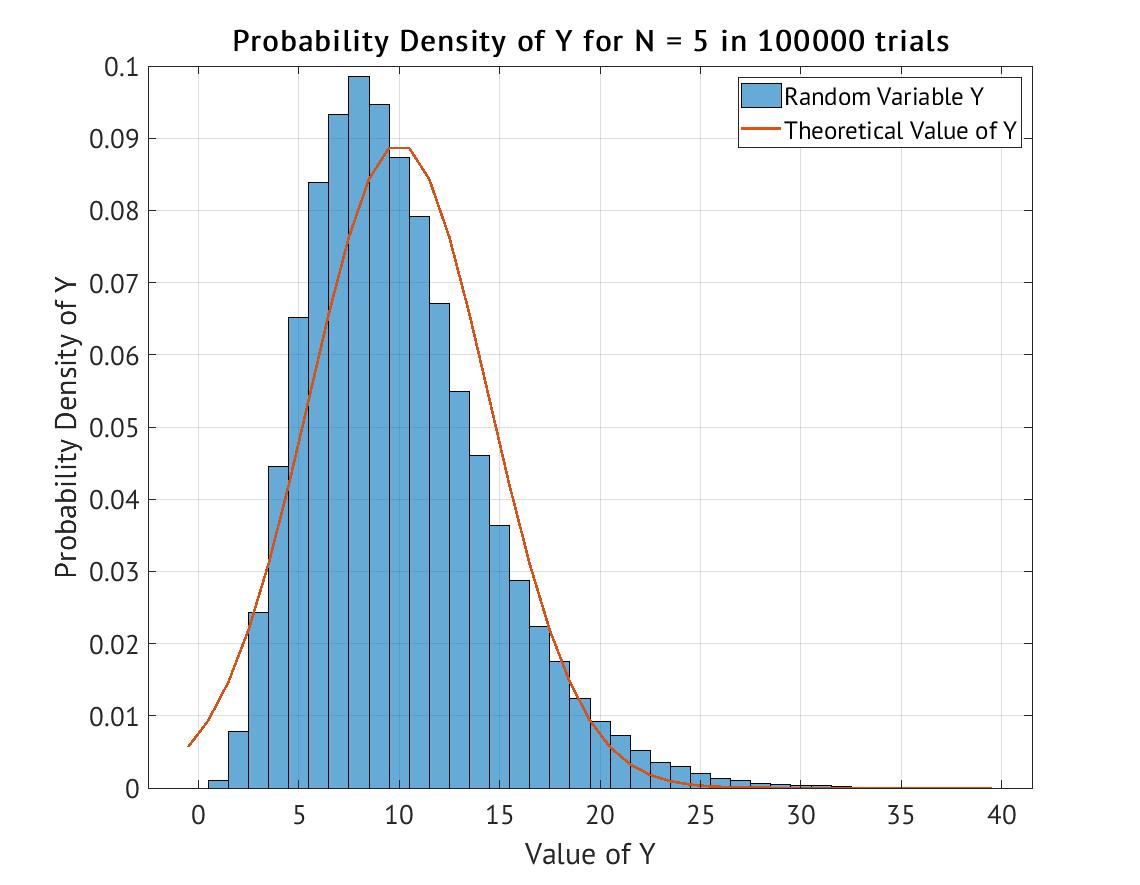
\includegraphics[width=0.5\textwidth]{./Images/ExpFig1.jpg} }}
    \subfloat[Sum of 50 Exponential Distributions]{{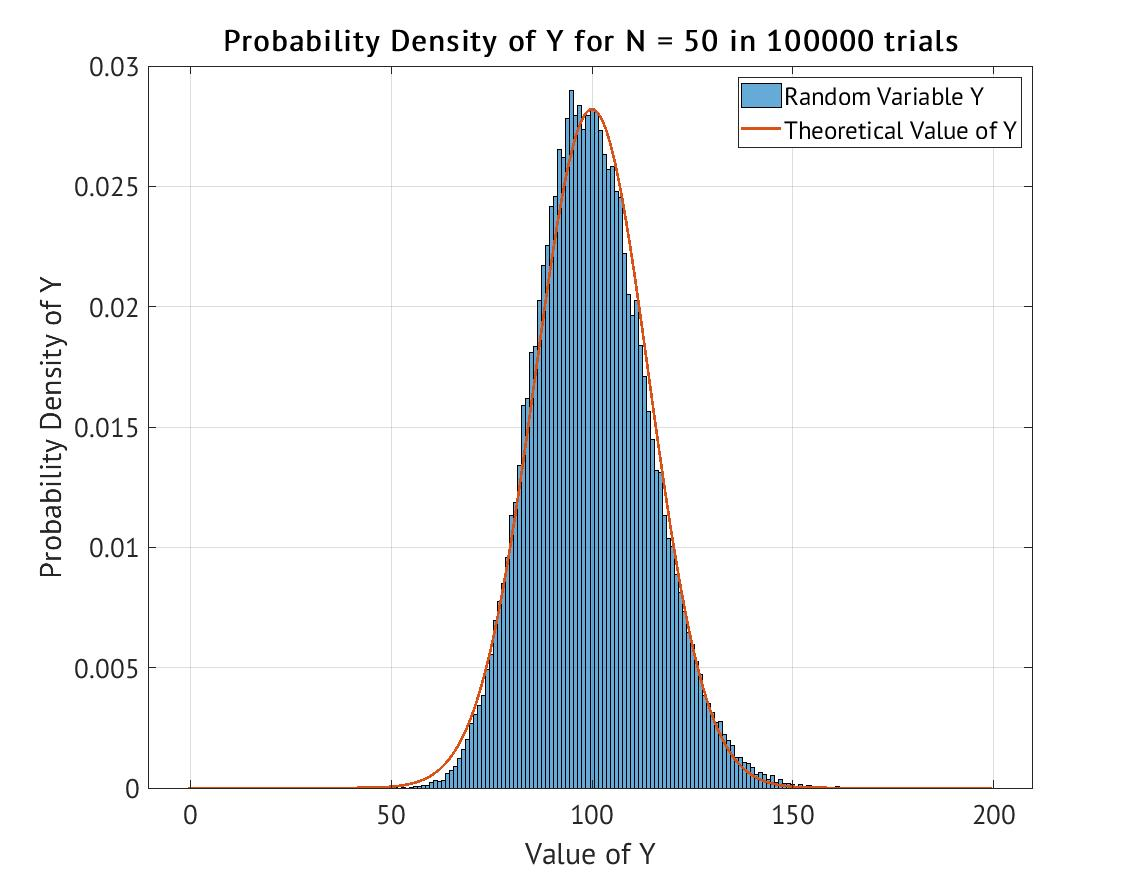
\includegraphics[width=0.5\textwidth]{./Images/ExpFig2.jpg} }} \\
    \subfloat[Sum of 150 Exponential Distributions]{{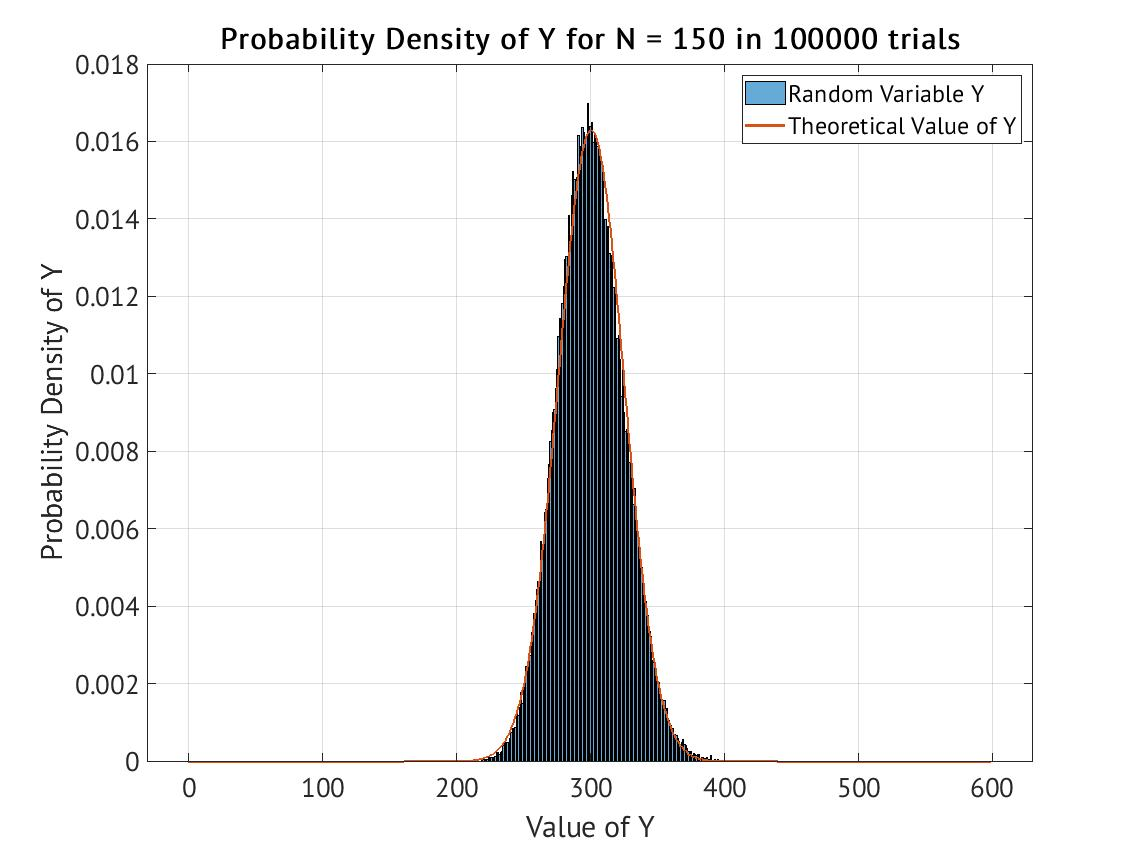
\includegraphics[width=0.5\textwidth]{./Images/ExpFig3.jpg} }}
\caption{\label{fig:ExpSubFig}Sum of iid Exponential Random Variables for N = 5,50,150}
\end{figure}

\medskip
\noindent
Contrasting this case to that of the former in Sections \ref{sec:org0023b57} and \ref{sec:org23375f9} where after just a small amount of sums the analytical and simulated outputs are very very close.
With this case there is a much larger difference that takes many more iterations to reach something that is more like the analytical shown as the orange line.

\noindent
In each subfigure of Figure \ref{fig:ExpSubFig} there is a discontinuity at \(Y = 0\), as that is an artifact similar to that of the previous section, where the sum of \(N\) random variables cannot go below \(0\) as there are bounds on the domain of the defining function.

\medskip
\noindent
The mean of an exponential distribution is commonly known as \(\displaystyle\frac{1}{\lambda}\), and similarly the variance is known as \(\displaystyle\frac{1}{\lambda^2}\). In each case shown in Figure \ref{fig:ExpSubFig}, these common values are multiplied by the corresponding value of \(N\).
This shows the connection and use of the CLT in this case.

\medskip
\noindent
The Gaussian plot overlayed on the histograms uses the above common mean and variance to calculate each specific mean and variance. In each case, as \(N\) gets larger the approximation is better and better, leading to a more accurate description.

\medskip
\noindent
The mean and variance are calculated using the methods similar to those in the previous sections. The analytical and the simulated values of each are enumerated below in Table \ref{tab:ExpTable}.

\begin{table}[htbp]
\caption{\label{tab:ExpTable}Simulated and Analytical Mean and Variance for each trial of N}
\centering
\begin{tabular}{|c|c|c|c|c|}
\hline
N & Analytical Mean & Simulated Mean & Analytical Variance & Simulated Variance\\
\hline
5 & 10 & 9.9853 & 20 & 20.0472\\
50 & 100 & 99.9916 & 200 & 198.3358\\
150 & 300 & 299.9169 & 600 & 598.6283\\
\hline
\end{tabular}
\end{table}



\subsection{Sum of Independent, Identically Distributed Bernoulli Trials}
\label{sec:org3bb145c}
This simulation is described as the sum of \(N\) iid Bernoulli trials. This is also known as a Binomial distribution with the form \(p^k(1-p)^{N-k}\), where \(N\) in this case is the same as \(N\) for the trials, and \(k\) is equivalent to the specific value within \(N\) that is being focused at the time.
The CLT still holds again in this case as the same situations reoccurred. Thus, in each graph of each subfigure of Figure \ref{fig:BernSubFig} both the PMF and PDF of each is shown.

\pagebreak
\begin{figure}
    \centering
    \subfloat[Sum of 4 Bernoulli Distributions]{{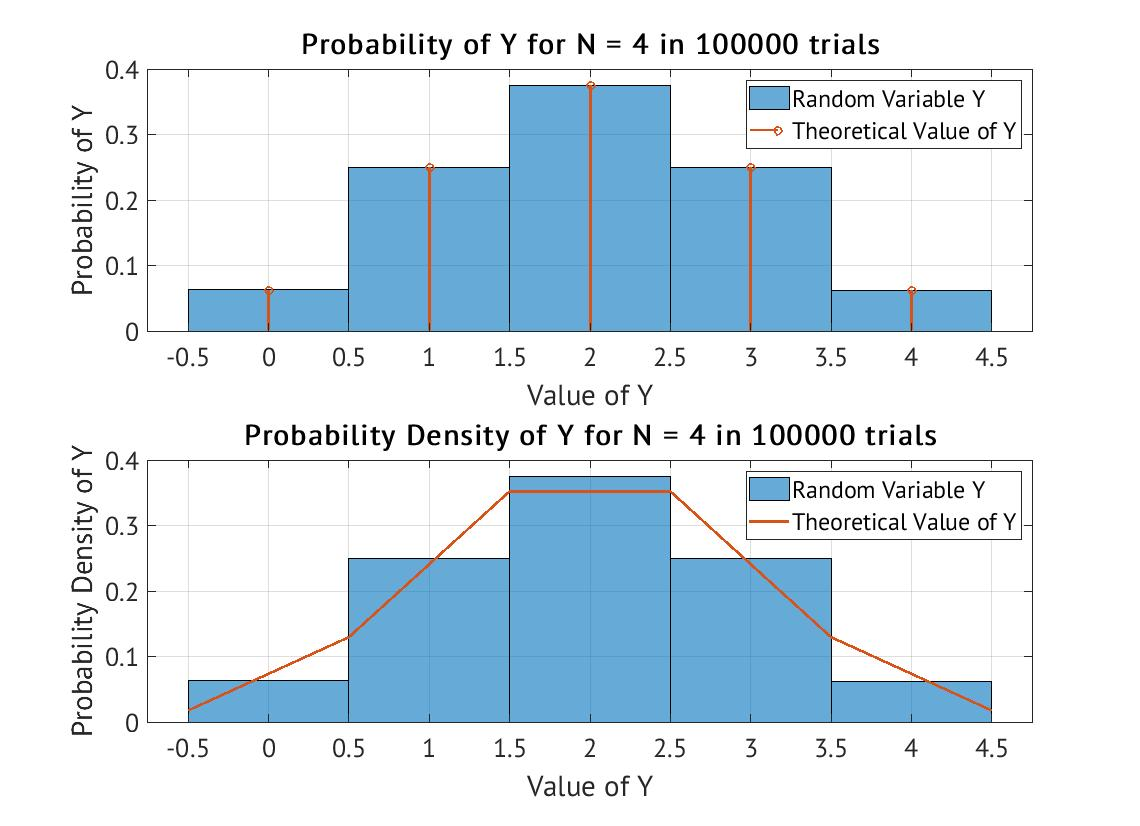
\includegraphics[width=0.5\textwidth]{./Images/BernFig1.jpg} }}
    \subfloat[Sum of 8 Bernoulli Distributions]{{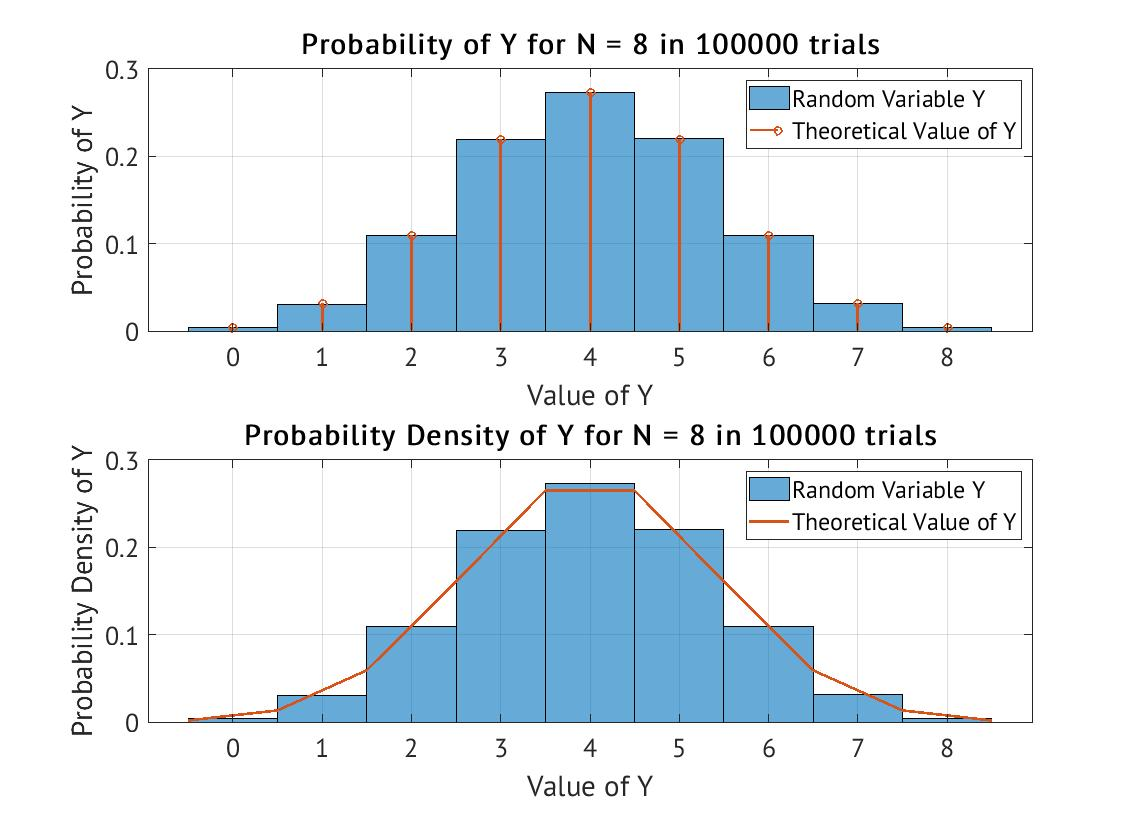
\includegraphics[width=0.5\textwidth]{./Images/BernFig2.jpg} }} \\
    \subfloat[Sum of 40 Bernoulli Distributions]{{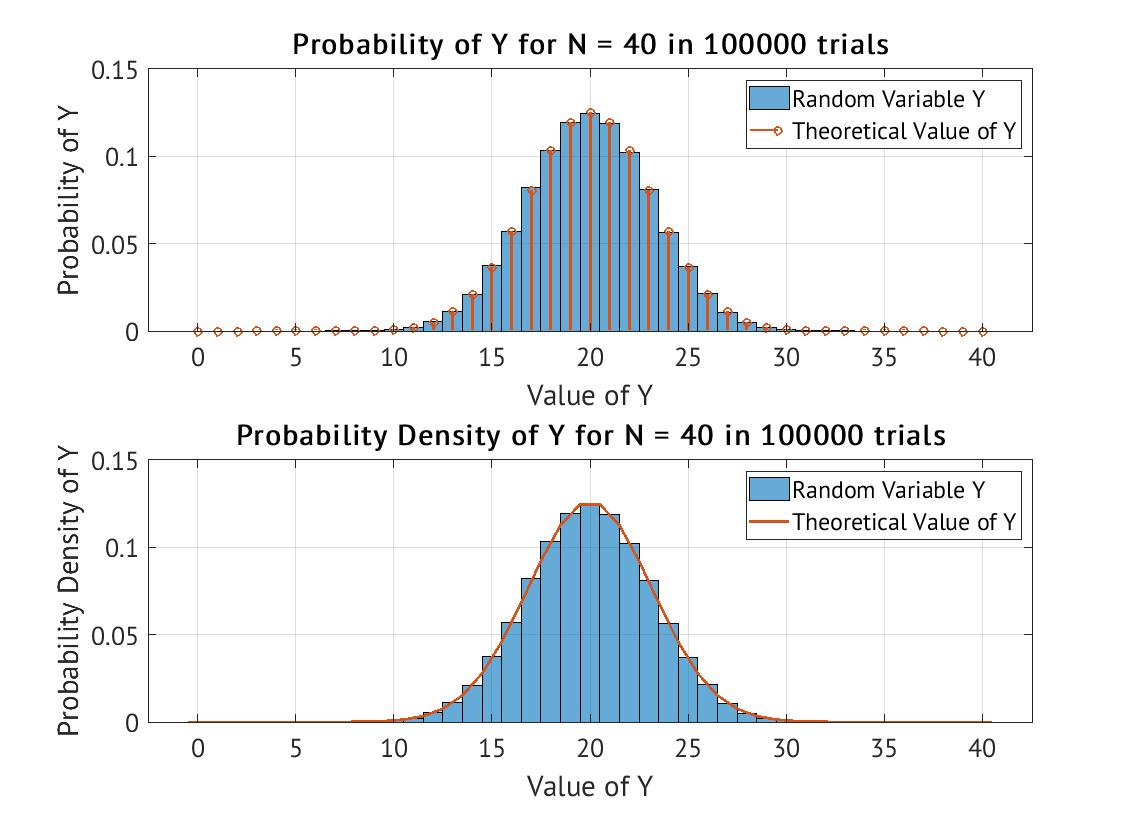
\includegraphics[width=0.5\textwidth]{./Images/BernFig3.jpg} }}
\caption{\label{fig:BernSubFig}Sum of iid Bernoulli Random Variables for N = 4,8,40}
\end{figure}


\medskip
\noindent
In each subfigure of Figure \ref{fig:BernSubFig} there is both the PDF and PMF of the given functions. There is little difference overall for each given that each histogram bin is the index of the first \(1\) being found within the generated trials. Thus, the PDF can only have an effective output when the bin width is \(1\) as well.
Either way, the PMF is a Binomial distribution based on being the sum of \(N\) trials of a Bernoulli simulation. In this case the given \(p\) is \(0.5\), thus giving an equal chance of \(0\) or \(1\).
Building on this, the Gaussian distribution in this case is shown to be the same as the Binomial for the given data (this point is also shown in the attached code).

\medskip
\noindent
The mean and variance of a Bernoulli distribution is given just as \(p\) for the mean, and \(p(1-p)\) for variance. Using the value of \(p\) provided the analytical values are \(0.5\) and \(0.25\) respectively.
These values are then multiplied by the value of \(N\) for each case, just the same as each of the other simulations.
In each subfigure of Figure \ref{fig:BernSubFig} the mean is very obviously placed at \(0.5 \times N\) and as \(N\) grows, the variance increases as expected. This shows once again the CLT holds true.


\medskip
\noindent
As stated above, the mean and variance were calculated as expected from the same methods as in each other section. The simulated values are compared against these analytical values in the below Table \ref{tab:BernTable}.

\begin{table}[htbp]
\caption{\label{tab:BernTable}Simulated and Analytical Mean and Variance for each trial of N}
\centering
\begin{tabular}{|c|c|c|c|c|}
\hline
N & Analytical Mean & Simulated Mean & Analytical Variance & Simulated Variance\\
\hline
4 & 2 & 1.9992 & 1 & 1.002\\
8 & 4 & 4.0049 & 2 & 1.9972\\
40 & 20 & 20.0069 & 10 & 10.055\\
\hline
\end{tabular}
\end{table}


\section{What was Learned}
\label{sec:orgc2fcf96}
This project entirely focuses on the CLT. Given this, the differences in each section are mostly superficial. This is due to the same, or a similar outcome, being the output of each section. That is the point of it all, but reinforces the idea of what the CLT is doing. The differences that are there between the functions comes more from the generation and the summation of the random variables, which makes sense, then the graphing is meant to show what the outcome of this is. Some of this seemingly gets obfuscated in the process, this is mostly seen in Sections \ref{sec:org69fa2f4} and \ref{sec:org3bb145c}.
What I mean by this is that there is some amount of the process that is a little vague just due to the conversion of Bernoulli to Gaussian/Binomial.

\medskip
\noindent
With all of this being said, the applications of the CLT is very obvious, in that as the amount of something increases, the mean increases along with it, as well as the variance, but the general shape is going to get closer and closer to a Gaussian distribution, which is generally very easy to approach and work with.
\subsection{Issues and Changes}
\label{sec:org7e37b8f}
In the process of doing this project the only real issue that was had was the somewhat vagueness of the last section in what actually is happening. Though, this is not really an issue with the actual project and more of an issue wrapping my head around the process itself. The outcome still generally makes sense from working with the data and the graphs.
Other than this, there is little that I feel that needs to be changed, the functions used to generate the different random variables feel like a good choice, and that they are different enough that general intuition can't be entirely trusted to find the result from that alone.

\medskip
\noindent
The amount of time that I spent on this project is somewhere in the ballpark of about \(10\) hours. This includes the writing of the document and the execution of the code. Overall, not the hardest project that has happened yet, but a much more straightforward view on what is occuring and being done.
\end{document}
